\documentclass{beamer}
\usepackage[utf8]{inputenc}
\usetheme{Madrid}
\usecolortheme{default}
\usepackage{amsmath,amssymb,amsfonts,amsthm}
\usepackage{txfonts}

\usepackage{gvv}
\usepackage{graphicx}
\usepackage{lmodern}
\setbeamertemplate{page number in head/foot}[totalframenumber]

\title{4.13.10}
\author{Aditya Mishra - EE25BTECH11005}
\date{October 3, 2025}

\begin{document}

\begin{frame}
\titlepage
\end{frame}

\begin{frame}{Question}
\[
\vec{A} = \myvec{-1\\-7},\quad
\vec{B} = \myvec{5\\1},\quad
\vec{C} = \myvec{1\\10}
\]
Equation of the internal bisector of $\angle ABC$.
\end{frame}

\begin{frame}{Solution}
\[
\text{Given lines } \vec{n}_1^{\top} \vec{x} = c_1, \quad \vec{n}_2^{\top} \vec{x} = c_2,
\]
\[
\text{Angle bisectors satisfy }
\frac{|\vec{n}_1^{\top} \vec{x} - c_1|}{\|\vec{n}_1\|}
= \frac{|\vec{n}_2^{\top} \vec{x} - c_2|}{\|\vec{n}_2\|}.
\]
\[
\Rightarrow \quad
\frac{\vec{n}_1^{\top} \vec{x} - c_1}{\|\vec{n}_1\|}
= \pm \frac{\vec{n}_2^{\top} \vec{x} - c_2}{\|\vec{n}_2\|}.
\]
\end{frame}

\begin{frame}{Solution}
\[
\text{Internal bisector: sign chosen so that for }
\vec{u} =
\frac{\vec{A}-\vec{B}}{\|\vec{A}-\vec{B}\|}
+
\frac{\vec{C}-\vec{B}}{\|\vec{C}-\vec{B}\|},
\quad

\text{we have }
\operatorname{sgn}(\vec{n}_1^{\top} \vec{u}) = -\operatorname{sgn}(\vec{n}_2^{\top} \vec{u})
\]

\text{Normals:}
\begin{align*}
\vec{n}_1 &= \myvec{-8\\6} \\
\vec{n}_2 &= \myvec{9\\4}
\end{align*}
\text{Norms:}
\begin{align*}
\|\vec{n}_1\| = 10 \\
\|\vec{n}_2\| = \sqrt{97}
\end{align*}
\end{frame}

\begin{frame}{Solution}
Equation of angle bisector:
\[
\frac{\vec{n}_1^{\top} (\vec{x} - \vec{B})}{10}
=
-\frac{\vec{n}_2^{\top} (\vec{x} - \vec{B})}{\sqrt{97}}
\]
\[
\sqrt{97}\,\vec{n}_1^{\top} (\vec{x} - \vec{B}) + 10\,\vec{n}_2^{\top} (\vec{x} - \vec{B}) = 0
\]
\end{frame}

\begin{frame}{Solution}
With
$\vec{B} = \myvec{5\\1}$, equation of Angle Bisector is:
\[
\boxed{ \myvec{90-8\sqrt{97} \ 40+6\sqrt{97}}^T \vec{x} + (34\sqrt{97}-490) = 0 }
\]
\text{Or,}
\[
\boxed{\vec{x} = \myvec{5 \\ 1} + \lambda\myvec{40+6\sqrt{97} \\ -(90-8\sqrt{97})},\quad \lambda \in \mathbb{R}}
\]
\end{frame}


\begin{frame}{Plot}
\begin{figure}
    \centering
    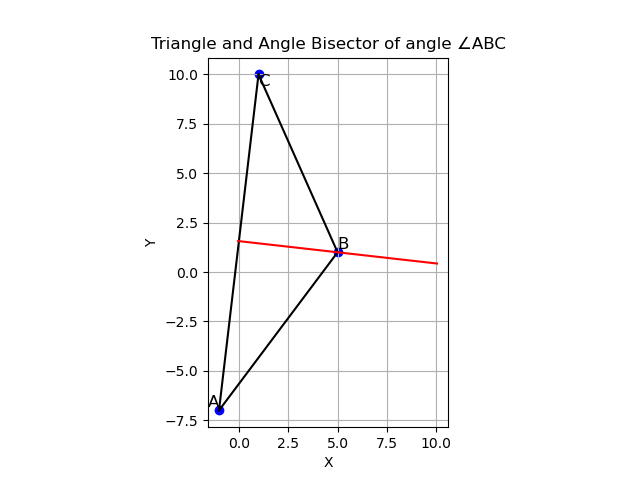
\includegraphics[width=0.8\columnwidth]{Figs/Figure_1.png}
\end{figure}
\end{frame}
\begin{frame}{Codes}
\centering
For Codes, refer to the URL below:  
\url{https://github.com/Aditya-Mishra11005/ee1030-2025/tree/temp/ee25btech11005/matgeo/4.13.10/Codes}
\end{frame}\end{document}

